% $Id$
\documentclass[twocolumn,prd,nofootinbib]{revtex4}


\newcommand\ForInternalReference[1]{}
\newcommand\SkipForEarlyCirculation[1]{}
\newcommand\AddedResponse[1]{{\color{blue} {#1}}}
%\newcommand\SkipForEarlyCirculation[1]{#1}
\newcommand\SkipPP[1]{}
\usepackage{verbatim}
\usepackage{graphicx}
\usepackage{dcolumn}
\usepackage{bm}
\usepackage{color}
\usepackage{xspace}
\usepackage{url}
\usepackage{amsmath}
%\usepackage{adjustbox}
\usepackage{float}
\usepackage{multirow}
%
%
\usepackage{times}
%
%
%
\newcommand\optional[1]{}

%
\newcommand\E[1]{\left\langle #1\right\rangle}
\newcommand\qmstate[1]{\left|#1\right \rangle}
\newcommand\qmstateKet[1]{\left\langle#1\right|}
\newcommand\qmstateproduct[2]{\left\langle#1|#2\right\rangle}
\newcommand\qmoperatorelement[3]{\left\langle#1\left|#2\right|#3\right\rangle}
\newcommand\qmoperator[1]{{\bf #1}}
%
\newcommand\Y[1]{{{}_{#1}Y}}

\newcommand\lnL{ \ln {\cal L}}
\newcommand\lnLmarg{ \ln{\cal L}_{\rm marg}{}}
\newcommand\unit[1]{{\rm #1}}

\newcommand\rapidPEOrig{rapid\_pe1}
\newcommand\ILE{ILE}
\newcommand\editremark[1]{{\color{red} #1}}
%
%
%
\usepackage{color}
\definecolor{amber}{rgb}{1.0, 0.75, 0.0}
\definecolor{orange}{rgb}{1.0, 0.5, 0.0}
\definecolor{amaranth}{rgb}{0.9, 0.17, 0.31}
\def\fixme#1{\textcolor{red}{#1}}
\newcommand{\Richard}[1]{ {\color{blue}{#1}}}
\newcommand{\ros}[1]{ {\color{blue}{#1}}}
%

%

%
%
%
%
\graphicspath{{./figures/}}
\newcommand{\mc}{{\cal M}}
\newcommand{\Ms}{M_{\odot}}
\newcommand\LambdaTilde{\widetilde{\Lambda}}
\newcommand\DeltaLambdaTilde{\delta \widetilde{\Lambda}}
%
\def\ltsima{$\; \buildrel < \over \sim \;$}
\def\simlt{\lower.5ex\hbox{\ltsima}}
\def\gtsima{$\; \buildrel > \over \sim \;$}
\def\simgt{\lower.5ex\hbox{\gtsima}}

\newcommand\prx{Phys.~Rev.~X}
\def\aj{Astronomical Journal}                 %
\def\apj{Astrophysical Journal}                %
\def\apjl{Astrophysical Journal}             %
\def\pasj{PASJ}
\def\apjs{ApJS}              %
\def\mnras{MNRAS}            %
\def\prd{Phys.~Rev.~D}       %
\def\prl{Phys.~Rev.~Lett}    %
\def\cqg{Class.~Quant.~Grav.~}%
\def\araa{ARA\&A}             %
\def\nat{Nature}              %
\def\aap{A\&A}                %
\def\aapr{A\&A~Rev.~}    %
\def\pasp{PASP}    %
\def\sovast{Soviet Ast.}
%
%

\newcommand{\IMRPD}{\textsc{IMRPhenomD}\xspace}
\newcommand{\IMRPDT}{\textsc{IMRPhenomD\_NRTidal}\xspace}
\newcommand{\IMRP}{\textsc{IMRPhenomPv2}\xspace}
\newcommand{\SEOBP}{\textsc{SEOBNRv3}\xspace}
\newcommand{\SEOBA}{\textsc{SEOBNRv4}\xspace}
\newcommand{\SEOBAROM}{\textsc{SEOBNRv4\_ROM}\xspace}
\newcommand{\NRSur}{NRSur7dq2\xspace}
\newcommand{\TEOB}{SEOBNRv4T\xspace}
\newcommand{\Resum}{TEOBResumS\xspace}
\newcommand\RIFT{RIFT}
\newcommand{\Taylor}{TaylorF2\xspace}
\newcommand\PaperDetection{\underline{LVC-detect}\cite{DiscoveryPaper}}
\newcommand\PaperPE{\underline{LVC-PE}\cite{PEPaper}}
\newcommand\PaperTestGR{\underline{LVC-TestGR}\cite{TestingGRPaper}}
\newcommand\PaperPENRMethods{\underline{PE+NR-Methods}\cite{gwastro-PENR-Methods-Lange}}
\newcommand\PaperAstro{\underline{LVC-Astro}\cite{AstroPaper}}
\newcommand\PaperBurst{\underline{LVC-Burst}\cite{BurstPaper}}
\newcommand\PaperRates{\underline{LVC-Rates}\cite{RatesPaper}}
\newcommand\PaperStochastic{\underline{LVC-Stochastic}}
\newcommand\PaperSEOBNRvthree{\underline{LVC-SEOBNRv3}\cite{SEOBv3Paper}}

\def\RIT{Center for Computational Relativity and Gravitation, Rochester Institute of Technology, Rochester, New York 14623, USA}

\begin{document}

\title{Population Inference of Eccentric Binary Black Holes}
\author{M. Zeeshan}
\affiliation{\RIT}
\author{R. O'Shaughnessy}
\affiliation{\RIT}
\begin{abstract}
Yet to work. 
\end{abstract}
\maketitle

\section{Introduction}
The Advanced LIGO  \cite{2015CQGra..32g4001T}  and Virgo \cite{gw-detectors-Virgo-original-preferred}  ground-based gravitational wave (GW) detectors have
identified several coalescing compact binaries
\cite{DiscoveryPaper,LIGO-O1-BBH,2017PhRvL.118v1101A,LIGO-GW170814,LIGO-GW170608,LIGO-GW170817-bns}.  
%



\section{Methods}
\label{sec:methods}

The Binary Black Holes (BBHs) can be described by three intrinsic and seven extrinsic parameters. The intrinsic parameters: such as mass ($m_i$), spin $( \chi_i)$, and eccentricity $(e)$, are subject to the orbital evolution of the binary. The extrinsic parameters: orientation (orbital phase, polarization, and inclination), sky location (right ascension, declination), luminosity distance, and coalescence time depend on the observer.

{\color{red}Most of the eccentric binaries are driven by low mass events \cite{?}}. Therefore,  in this study, we  will consider modest masses $(1M_\odot-40M_\odot)$, non-spinning $(\chi_i = 0)$, and eccentric $(0-1)$ binaries. In addition, we will use mass ratio $q=m_1/m_2$ with condition $m_1>m_2$ and total mass $M=m_1+m_2$. 



\subsection{Power law Model}




\begin{align}
\label{eq:plaw}
p(m_1,m_2,e) = &C(\alpha,m_{min},m_{max},M_{max},e)  
\nonumber \\ & \frac{m_1^{-\alpha}}{(m_1-m_{min})\sigma_e} 
\nonumber \\ &
\sqrt{\frac{2}{\pi}} e^{(-1/2)(e/\sigma_e)^2}
\end{align}

   



% \begin{align} \label{eq:strain_mode}
% h(t,\vartheta,\phi;\bm{\lambda}) = 
% \sum_{\ell=2}^{\infty} \sum_{m=-\ell}^{\ell} \frac{D_{\rm ref}}{D} h^{\ell m}(t;\bm{\lambda}) \Y{-2}_{\ell m} \left(\vartheta, \phi \right) \, ,
% \end{align}


% \begin{widetext}
% \begin{align}
% \ln {\cal L}(\bm{\lambda}, \theta) 
% &= (D_{\rm ref}/D) \text{Re} \sum_k \sum_{\ell m}(F_k \Y{-2}_{\ell m})^* Q_{k,lm}(\bm{\lambda},t_k)\nonumber \\
% &   -\frac{(D_{\rm ref}/D)^2}{4}\sum_k \sum_{\ell m \ell' m'}
% \left[
% {
% |F_k|^2 [\Y{-2}_{\ell m}]^*\Y{-2}_{\ell'm'} U_{k,\ell m,\ell' m'}(\bm{\lambda})
% }
% % \right. \nonumber \\ & \left.
%  {
% +  \text{Re} \left( F_k^2 \Y{-2}_{\ell m} \Y{-2}_{\ell'm'} V_{k,\ell m,\ell'm'} \right)
% }
% \right]
% \label{eq:def:lnL:Decomposed}
% \end{align}
% \end{widetext}

% \begin{eqnarray}
% {\cal L}_{\rm margT} \equiv  \int {\cal L} \frac{dt}{T}
% \label{eq:lnL:tmarg}
% \end{eqnarray}












% \begin{table*}
% \begin{tabular}{lrr|ccccc|rr}
% Version & srate & modes & $\tau_{start}$ & $\tau_{setup}$ & $\tau_{ad}$ & $\tau_{it,like}$ &$\tau_{it,rest}$ &
% $\frac{T_{ILE}}{N_{eval}}$ & GPU \\  %\hline 
%   &   Hz & m & sec & sec & & $\mu$sec & $\mu$sec  &sec  & use  \%\\ \hline 
% % ~/parse_report.sh profile_nogpu_pcdev13.log | more
% CPU & 16384 & $\pm 2 $ & 20 & 2.4 &&540 & 20 &  690  \\ 
%        & 4096 & $\pm 2 $ &   20  &&&& 20 \\ \hline
% % ./parse_report.sh 20190130-profile_nogpu_HM_pcdev13.log  | more
% % /parse_report.sh ./profile_nogpu_HM_lowres_pcdev13.log 
% %    setup time: PrecomputeLikelihoodTerms, includes waveform generation. 
% %   evaluation: FactoredLogLikelihodTimeMarginalized Divide by actual number of calls, since not a block!
% %    
% CPU & 16384 & $\pm 2,\pm 1 $ & 20 & 1.5 && 680 & 20 &  1060  \\ 
%        & 4096 & $ \pm 2, \pm 1 $ &   20 &&&& 20  \\ \hline

%GPU (a) & 16384 & $\pm 2 $  & 20  & & && & 270 \\
%            & 4096 &$\pm 2 $  &  20 &  & & & & 45 \\ \hline

%GPU (b) & 16384 & $\pm 2$ & 20  & 1.8 & 1 & 0.85& 20 &28 & 15\\
%        & 4096 & $\pm 2$  & 20 & $1.2 $ &  1  & 0.75 & 20  & 25\\ \hline

% GPU (b) & 16384 & $\pm 2, \pm 1$ & 20 & 1 && 4.2 & 20  & 38  \\
%        & 4096 & $\pm 2, \pm 1$ & 20 & 1&& 2.5  & 20 & 35 & \\ \hline

% GPU (c) & 16384 & $\pm 2 $  & 20  &6  & & 18&  58&160 &  \\
%             & 4096 &$\pm 2 $  &  20 & 3.7 & & 11  & 58  & 140 & $\simeq 50$ \\
% \end{tabular}
% Compute node at LIGO-WA
% \caption{\label{tab:CostBreakdown}\textbf{Profiling performance: Binary black holes}: Evaluation costs for the
%   marginalized likelihood on default
%   hardware, for a two-mode system $(l,m)=\pm 2$ analyzing $T=8\unit{s}$ of data with a massive binary black hole
%   $m_1=35 M_\odot,M_2=30 M_\odot$.  The last column indicates peak GPU utilization.
% }
%\end{table*}










% \subsection{Binary black hole analysis}
% \label{sec:sub:BBHFull}

% \begin{figure*}

% 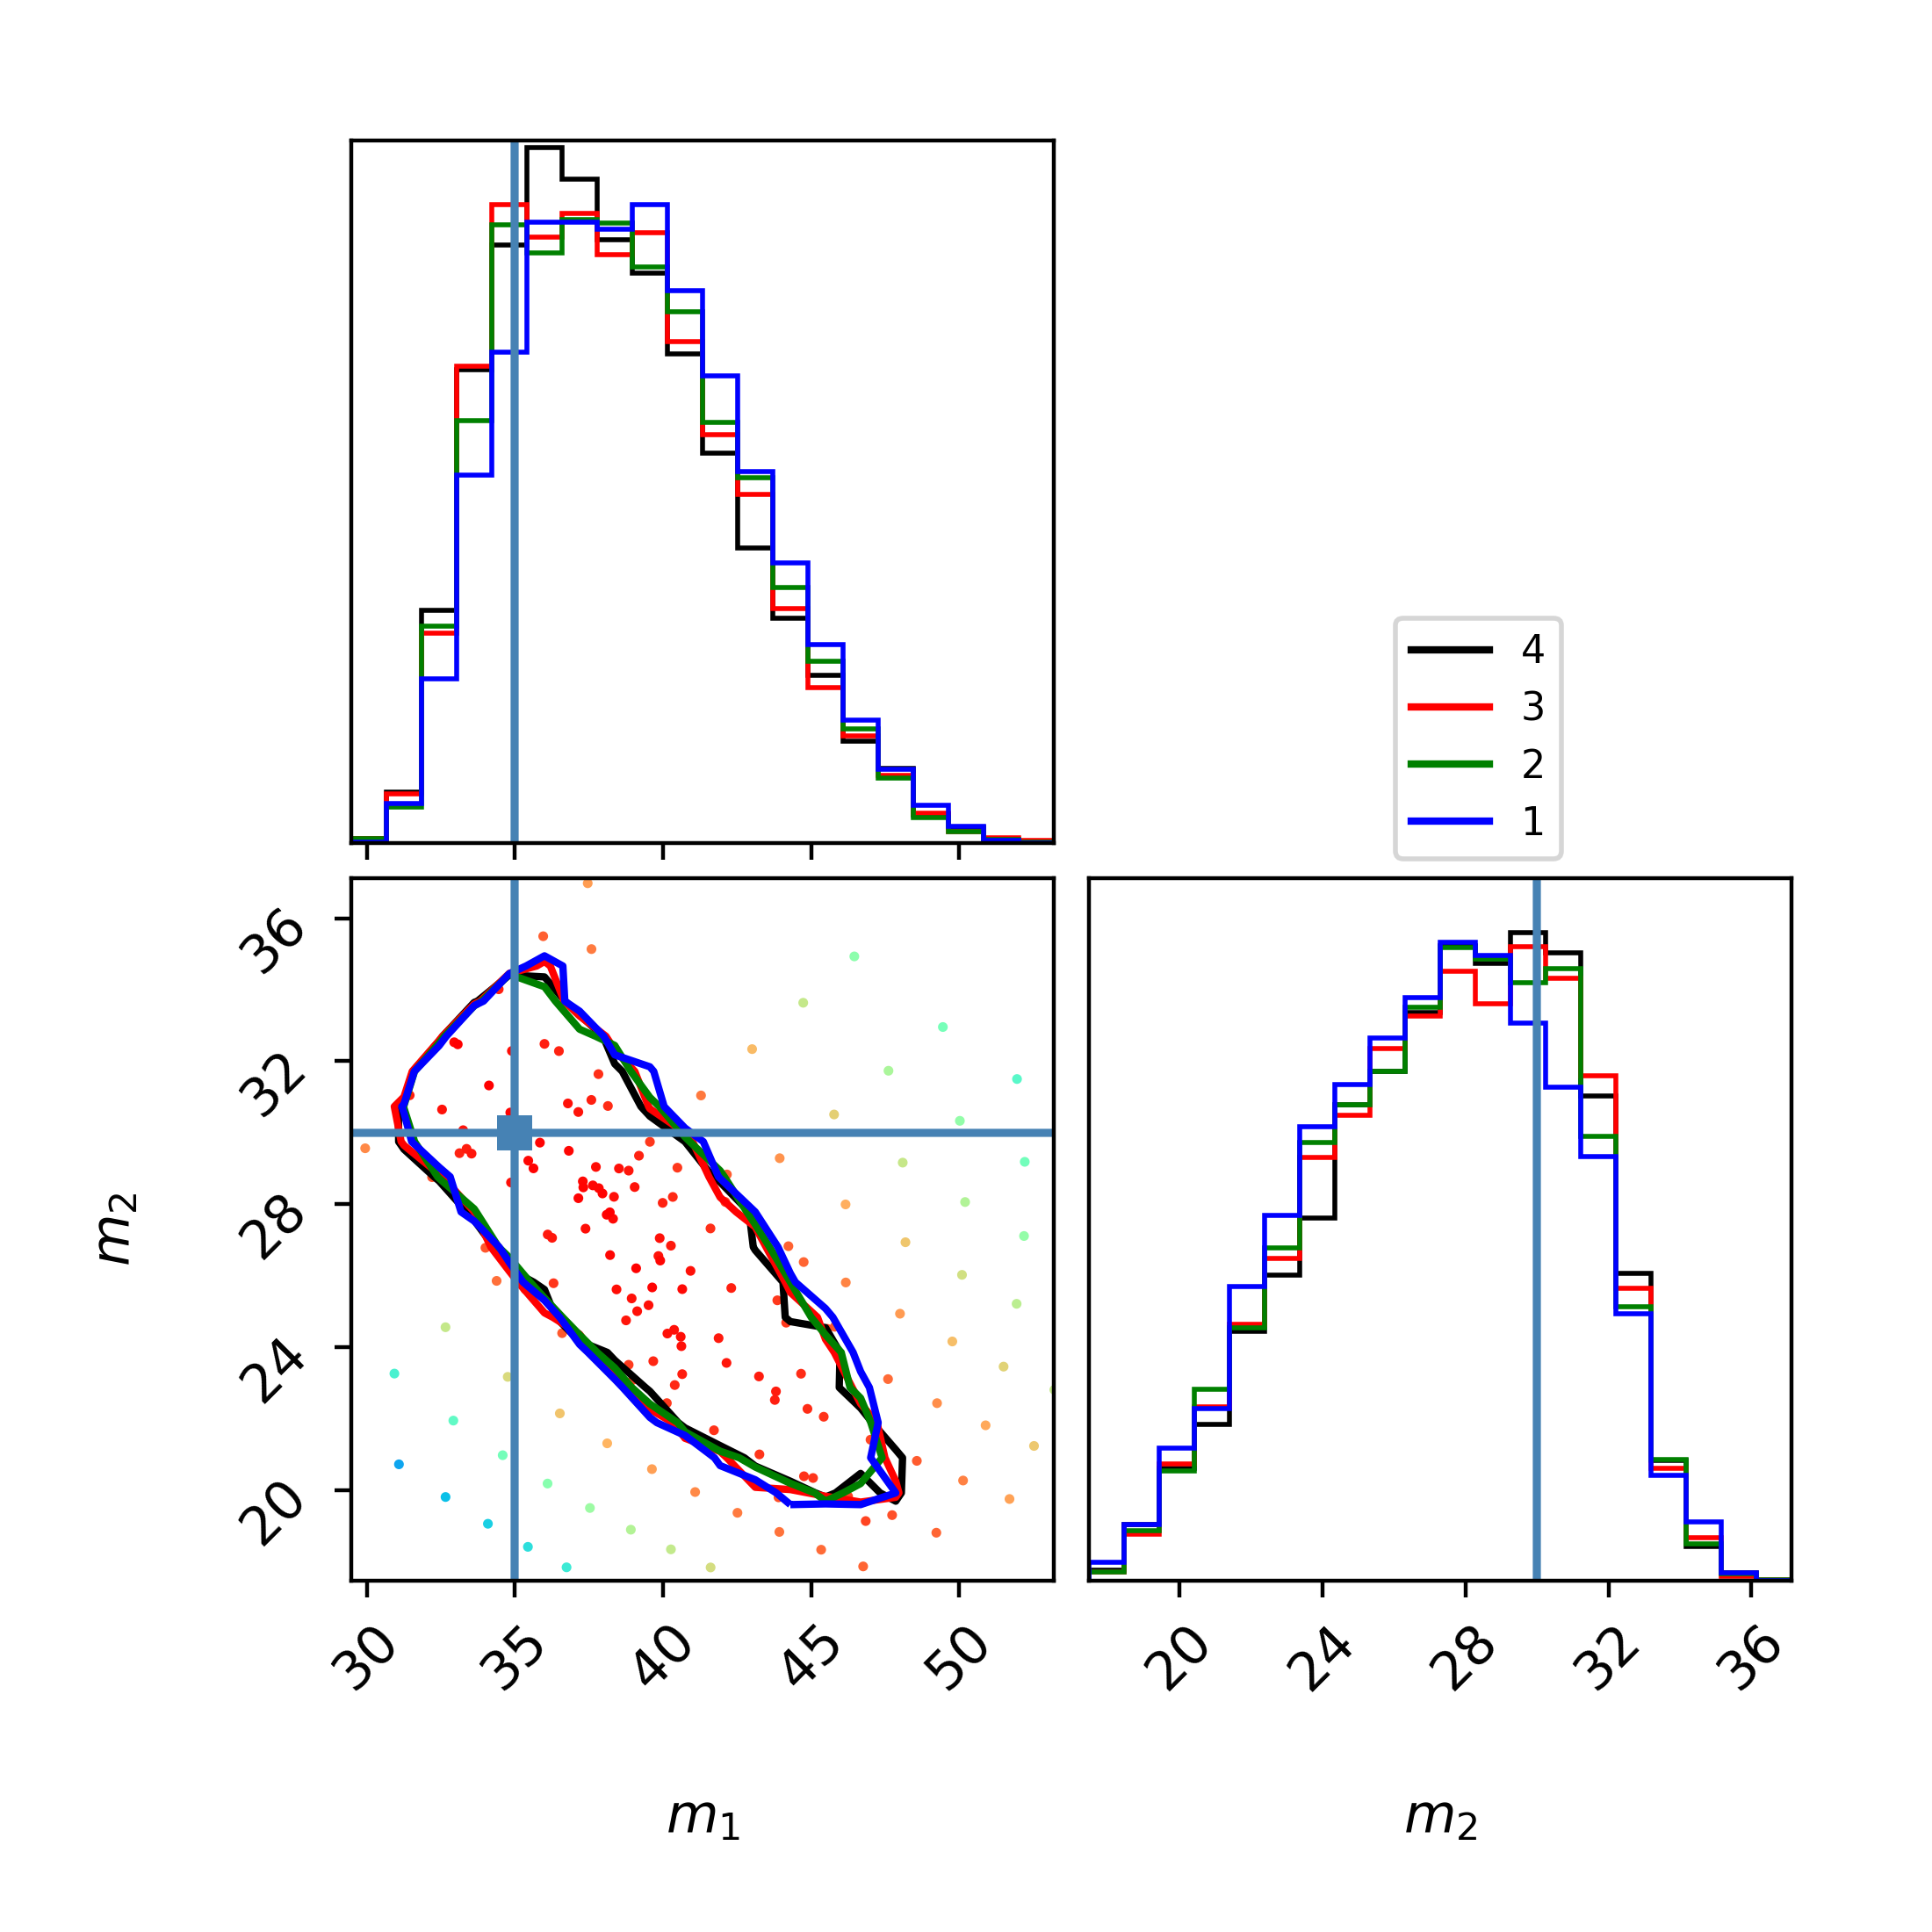
\includegraphics[width=0.45\textwidth]{figures/bbh_zerospin_m1_m2.png}
% 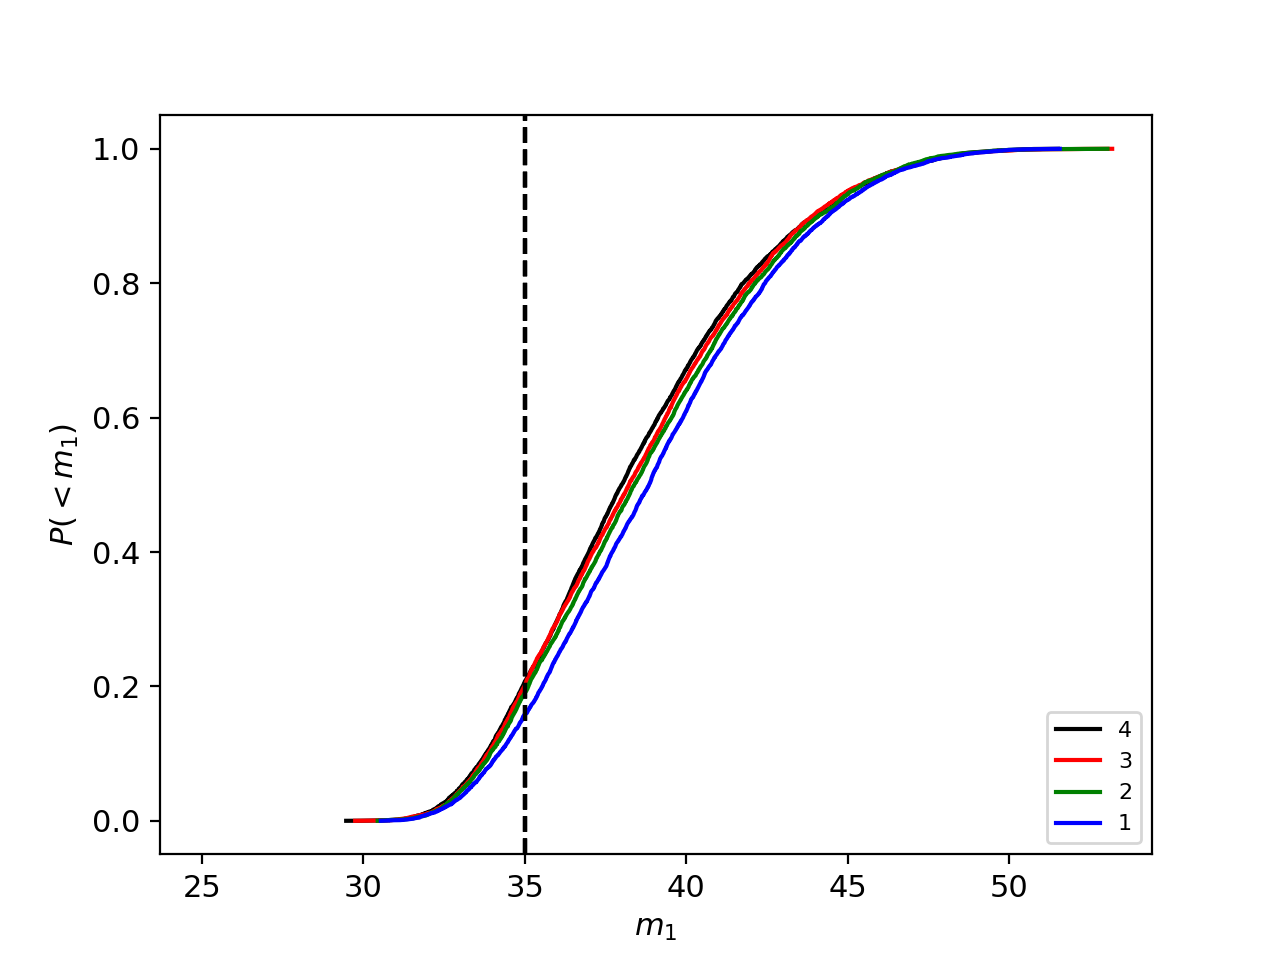
\includegraphics[width=0.45\textwidth]{figures/bbh_zerospin_m1_cum.png}
% % python plot_mean_variance.py --convergence-file 20190203-bbh-zerospin-batch_gpu_lowlatency_meanVar.dat  --output bbh_zerospin_lnL_meanVar
% 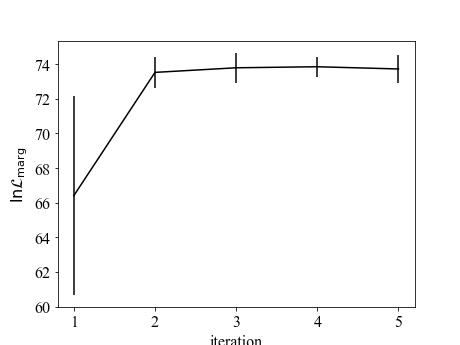
\includegraphics[width=0.45\textwidth]{figures/bbh_zerospin_lnL_meanVar.png}
% % python plot_convergence.py --convergence-file 20190203-bbh-zerospin-batch_gpu_lowlatency.dat
% 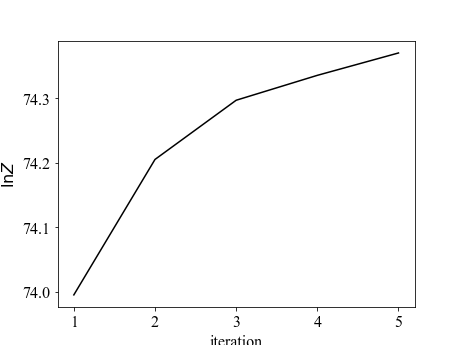
\includegraphics[width=0.45\textwidth]{figures/bbh_zerospin_lnL_converge.png}
% \caption{\label{fig:BBH:MultiIterate}\textbf{Convergence of BBH analysis: Zero spin}: Results for marginal posterior distributions
%   of our fiducial synthetic binary black hole.  Solid contours show credible intervals; solid one-dimensional distributions
%   show marginal CDFs and PDFs for the corresponding variable; and colored points indicate the location $\bm{\lambda}$ and
%   value of the underlying marginalized likelihood evaluations.   
% %The corresponding dotted curves show an analysis using   only the $m=\pm 2$ modes \editremark{perform both} 
% \emph{Left panel } Posterior distribution
%   over  $\mc$ and
%   $\delta=(m_1-m_2)/M$.    \emph{Right panel}: Marginal 1d CDFs of $\mc$, showing convergence.
% \emph{Bottom left}: Mean and variance of  \AddedResponse{the array $\ln{\cal L}_{\rm marg}(\bm{\lambda}_j)$  for
% $j=1,2,\ldots N_{\rm eval}$ indexing all candidate sets of intrinsic parameters $\bm{\lambda}_j$ performed in that iteration},  showing that after the
% first iteration the
% candidate points are consistent with the posterior (i.e., no proposed point has very low $\ln {\cal L}_{\rm marg}$).
% \emph{Bottom right panel}: The estimated evidence $Z = \int d\bm{\lambda} {\cal L}_{\rm marg}$ versus iteration number.  As systematic fitting error dominates our
% error budget, Monte Carlo error is not shown.
% }
% \end{figure*}


















\section{Conclusions}
\label{sec:conclude}
In Progress, 













\begin{acknowledgements}
We thank our anonymous referee for the helpful feedback.

\end{acknowledgements}


\appendix
In Progress,




%\bibstyle{unsrt}
\bibliography{paperexport,LIGO-publications}
\end{document}
